\documentclass[13.5pt]{beamer}

% Presento style file
\usepackage{config/presento}

% custom command and packages
\input{config/custom-command}

% Information
\title{Quantum Chromatic Number of a Graph}
\subtitle{}
\author[Fabian]{Felix Kirschner, Simon Nietz, Fabian Portner}
\institute{THP, Universität zu Köln}
\date{Block Seminar on Numerical Optimization and Quantum Information \\ August 8, 2017}
\setbeamertemplate{headline}
{%
\begin{beamercolorbox}{section in head/foot}
\vskip2pt\insertnavigation{\paperwidth}\vskip2pt
\end{beamercolorbox}%
}
\setbeamertemplate{section in head/foot shaded}[default][20]

\begin{document}

% Title page
\begin{frame}[plain]
\maketitle
\end{frame}


% sections in the presentation
\section{Motivation}
\begin{frame}{Messages from Aliens}
\begin{columns}[t]
\begin{column}{0.4\textwidth}
\includegraphics[height=5.5cm]{images/et.jpg} \pause
\end{column}
\begin{column}{0.25\textwidth}
\begin{tikzpicture}
\draw[->, >=stealth',decorate, thick, colororange, decoration=snake] (0,1) -- (1.5,1);
\draw[->, >=stealth',decorate, thick, colororange, decoration=snake] (0,2)-- (1.5,2);
\draw[->, >=stealth',decorate, thick, colororange, decoration=snake] (0,3)-- (1.5,3);
\node  at (0.75,3.5) {\%6\#7k$\rightarrow$\$};
\node  at (0.75,2.5) {g$\uparrow$ k$\leftarrow$f\$};
\node  at (0.75,1.5) {u!+\&j+-+};
\end{tikzpicture}
\end{column}
\begin{column}{0.4\textwidth}
\includegraphics[height=5.5cm]{images/seti.jpg}
\end{column}
\end{columns}
\end{frame}






\begin{frame} {Entanglement as resource}
\scalebox{0.8}{
\begin{tikzpicture}
	\node[block] (b) {Faster computation};
    \node[block, below =1.5cm of b] (c) {Less electricity usage / carbon footprint};
    \draw[line] (b.south) -- (c.north);
    \node[block, below =1.5cm of c] (d) {Save lives \& still search for aliens};
    \draw[line] (c.south) -- (d.north); \pause
    \node[block, left =2cm of b] (a) {Quantum entanglement};
    \draw[line] (a.east) -- (b.west); \pause
    \node[right = 1cm of d] {\Cooley[5][colorblue]};
\end{tikzpicture}}
\end{frame}









\section{Introduction}
\begin{frame}{QM Crash Course}
\begin{block}{\color{colorblue}\textbf{Setting}}
\begin{itemize}
\item[$\bullet$] States are normalized elements $\ket{\phi}$ in an abstract, complex Hilbert space $\mathcal{H}$ \pause
\item[$\bullet$] The composite space of two systems is $\mathcal{H}_1 \otimes \mathcal{H}_2$
\end{itemize}
\end{block}

\centering
  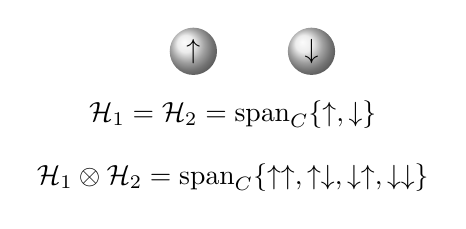
\begin{tikzpicture}
      % electrons
    \shade[ball color=gray!20] (-0.5,2) coordinate(Hp) circle (.3) node {$\uparrow$};
    \shade[ball color=gray!20] (1,2) coordinate(Hp) circle (.3)node {$\downarrow$};
    \node at (0,1.2) {$\mathcal{H}_1 = \mathcal{H}_2 = \mathrm{span}_{\mathbb{C}}\{ \ket{\uparrow}, \ket{\downarrow} \}$ };
    \node at (0,0.4) {$\mathcal{H}_1 \otimes \mathcal{H}_2 = \mathrm{span}_{\mathbb{C}} \{ \ket{\uparrow \uparrow }, \ket{\uparrow \downarrow}, \ket{\downarrow \uparrow }, \ket{\downarrow \downarrow} \}  $};
  \end{tikzpicture} \pause
\begin{itemize}
\item[$\bullet$] Entangled states can \textbf{not} be written as $\ket{\psi} = \ket{\phi_1} \otimes \ket{\phi_2}$ with $\ket{\phi_i} \in \mathcal{H}_i$ 
\end{itemize}
\end{frame}

\begin{frame} {QM Crash Course}
\begin{block}{\color{colorblue}\textbf{Observables and Measurements}}
\begin{itemize}
\item[$\bullet$] Observables are self-adjoint operators  $O \in \mathrm{End}(\mathcal{H})$ with Eigensystem $\{ \lambda_i, \ket{\psi_i} \}$ \pause
\item[$\bullet$] With $\bra{\phi} = \braket{\phi , \cdot}$ we can write $O = \sum_i  \lambda_i \ket{\psi_i}\bra{\psi_i}$ 
\item[$\bullet$] The projections $E_i = \ket{\psi_i}\bra{\psi_i}$ are the measurement operators \pause
\item[$\bullet$] measurement operators fulfill: $E_i \geq 0$, $\sum_i E_i = I$, $E_i^2=E_i$ \pause
\item[$\bullet$] Measuring a state $\ket{\phi}$ yields observable $\lambda_i$ with probability $P_i = |\braket{\psi_i | \phi}|^2 = \bra{\phi} E_i \ket{\phi}$
\end{itemize} 
\end{block}
\end{frame}


\begin{frame}{GT Crash Course}
	\begin{tikzpicture}
    % spacing of tikz
    \draw (0,0) circle (0.0cm);
      \draw (5,2.5) circle (0.0cm);
    % graph
    \filldraw[fill=colororange!60!white, draw=black, thick] (4.8,2.2) circle (0.15cm);
    \filldraw[fill=colorgreen, draw=black, thick] (4.3,1.4) circle (0.15cm);
    \filldraw[fill=colorblue!60!white, draw=black, thick] (3.3,2) circle (0.15cm);
    \filldraw[fill=colororange!60!white, draw=black, thick] (2.5,2.4) circle (0.15cm);
    \filldraw[fill=colororange!60!white, draw=black, thick] (3.3,1.2) circle (0.15cm);

    \draw[vertex] (4.8, 2.2) -- (4.3, 1.4);
    \draw[vertex] (4.8, 2.2) -- (3.3, 2);
    \draw[vertex] (3.3,2) -- (3.3, 1.2);
    \draw[vertex] (3.3,2) -- (4.3, 1.4);
    \draw[vertex] (2.5,2.4) -- (3.3,2);
    \draw[vertex] (3.3,1.2) -- (4.3, 1.4);
    \node at (3.7,0.6) {$G=(V,E)$}; \node at (6.1, 1.6) {$\chi(G)=3$};
    \end{tikzpicture}
    
	\begin{itemize}
		\item[$\bullet$] A graph $G = (V,E)$ consists of vertices (points) $v \in V$ and edges 
        				$uv \in E$ that connect vertices $u$ and $v$.
        \item[$\bullet$] Connected vertices are called adjacent \pause
        \item[$\bullet$] A coloring is a map $f: V \to [c]=\{1,\dots,c \}$ such that 
        					$f(u) \neq f(v)$ if $uv \in E$.
        \item[$\bullet$] The smallest $c$ such that a coloring exists is called 
        				chromatic number $\chi(G)$             
	\end{itemize}
\end{frame}


\section{The Coloring Game}
\begin{frame}{The Coloring Game}

\begin{tikzpicture}
    % spacing of tikz
      \draw (-5,-2.5) circle (0.0cm);
      \draw (5,2.5) circle (0.0cm);
    % graph
    \filldraw[fill=colororange!60!white, draw=black, thick] (4.8,2.2) circle (0.15cm);
    \filldraw[fill=colorgreen, draw=black, thick] (4.3,1.4) circle (0.15cm);
    \filldraw[fill=colorblue!60!white, draw=black, thick] (3.3,2) circle (0.15cm);
    \filldraw[fill=colororange!60!white, draw=black, thick] (2.5,2.4) circle (0.15cm);
    \filldraw[fill=colororange!60!white, draw=black, thick] (3.3,1.2) circle (0.15cm);

    \draw[vertex] (4.8, 2.2) -- (4.3, 1.4);
    \draw[vertex] (4.8, 2.2) -- (3.3, 2);
    \draw[vertex] (3.3,2) -- (3.3, 1.2);
    \draw[vertex] (3.3,2) -- (4.3, 1.4);
    \draw[vertex] (2.5,2.4) -- (3.3,2);
    \draw[vertex] (3.3,1.2) -- (4.3, 1.4);
    \node at (3.7,0.6) {$G=(V,E)$};

    \node at (-4.8,1.7) {\Strichmaxerl[3][10][10][][]};
    \node at (-4.8,1) {Alice};

    \node at (-2.4,1.7) {\Strichmaxerl[3.5][][][][]};
    \node at (-2.4,1) {Referee};

    \node at (0,1.7) {\Strichmaxerl[3][-10][-10][][]};
    \node at (0,1) {Bob};

    \draw[thick, ->, shorten >=2pt, >=stealth'] (-4.8, 0.7) to [bend right=45] node[below] {\color{colorblue}\Large ${\alpha}$}  (-2.4, 0.7);

    \draw[thick, ->, shorten >=2pt, >=stealth'] (0, 0.7) to [bend left=45] node[below] {\color{colororange}\Large ${\beta}$} (-2.4, 0.7);

    \draw[thick, <-, shorten >=2pt, >=stealth'] (-4.8, 2.2) to [bend left=45] node[above] {\Large ${u}$} (-2.4, 2.2);

    \draw[thick, <-, shorten >=2pt, >=stealth'] (0, 2.2) to [bend right=45] node[above] {\Large ${v}$} (-2.4, 2.2);

    \node[llabel, rounded corners,fill=gray!20] at (0, -2) {To \textbf{win}, convince referee that they have c-coloring, i.e.:\\ \vspace{0.1cm} \hspace{0.2cm} (i) if $u=v$ then {\color{colorblue}$\alpha$} = {\color{colororange}$\beta$} \\ \vspace{0.1cm} \hspace{0.2cm}
    (ii) if $u v \in E$ then {\color{colorblue}$\alpha$} $\neq$ {\color{colororange}$\beta$}};


  \end{tikzpicture}
\end{frame}


\begin{frame}{The Quantum Coloring Game}

\begin{tikzpicture}
% spacing of tikz
  \draw (-5,-2.5) circle (0.0cm);
  \draw (5,2.5) circle (0.0cm);
  
%  Game
\node at (-4,2.2) {\Strichmaxerl[2.5][10][10][][]};
\node at (-4,1.5) {Alice};

\node at (4,2.2) {\Strichmaxerl[2.5][-10][-10][][]};
\node at (4,1.5) {Bob};

% Hilbert space
\node at (0,2) {\LARGE $\mathcal{H}_1 \otimes \mathcal{H}_2$};
\path (0,0.5) -- node[sloped] {\Large $\in$} (0,2);
\node at (0,0.5) {\large $\ket{\psi}$};
\node at (0,-0.2) {$\neq \ket{\varphi_1} \otimes \ket{\varphi_2}$};

% Measurements
\draw[thick, ->, shorten >=2pt, >=stealth'] (-4, 1.3) to [bend right=0] node[below,sloped] {\Large $E_{u,\color{colorblue}\alpha} \otimes I$} (-0.4, 0.5);
\draw[thick, ->, shorten >=2pt, >=stealth'] (4, 1.3) to [bend left=0] node[below,sloped] {\Large $I \otimes F_{v,\color{colororange}\beta}$} (0.4, 0.5);

% Infos 
\node[llabel, rounded corners,fill=gray!20] at (0, -2) {
Allow them to locally measure on an entangled product state.\\ 
They win without doubt, if: \\ \vspace{0.1cm} \hspace{0.2cm} (i) for all $u \in V$ and {\color{colorblue}$\alpha$} $\neq$ {\color{colororange}$\beta$} :
$\bra{\psi} E_{u, \color{colorblue}\alpha}  \otimes F_{u, \color{colororange}\beta} \ket{\psi} = 0$  
\\ \vspace{0.1cm} \hspace{0.2cm}
(ii) for all $uv \in E$ and {\color{colorblue}$\alpha$}:
$\bra{\psi} E_{u, \color{colorblue}\alpha}  \otimes F_{v, \color{colorblue}\alpha} \ket{\psi} = 0$};

  \end{tikzpicture}
\end{frame}


\begin{frame}{The Quantum Chromatic Number}
\begin{block}{\color{colorblue}\textbf{Idea}}
\vspace{0.1cm}
Instead of fixing c-coloring beforehand, answer with measurement results, numbered by {\color{colorblue}$\alpha$} and {\color{colororange}$\beta$} ($\in [c] = \{1,\dots,c\}$).
\end{block}

\begin{block}{\color{colorblue}\textbf{Definition}}
\vspace{0.1cm}
Quantum Chromatic Number $\chi_q(G)$ is the smallest possible $c$ to win the game without doubt.
\end{block}

\end{frame}

\begin{frame}{Example}

\begin{tikzpicture}
% spacing of tikz
  \draw (-5,-2.5) circle (0.0cm);
  \draw (5,2.5) circle (0.0cm);
  
% graph
\filldraw[fill=colororange!60!white, draw=black, thick] (4.8,2.2) circle (0.15cm);
\filldraw[fill=colorgreen, draw=black, thick] (3.5,2.2) circle (0.15cm);
\draw[vertex] (4.8, 2.2) -- (3.5, 2.2);
\node at (4.2,1.5) {$G=(V,E)$};

% electrons
\shade[ball color=gray!20] (-2.5,2) coordinate(Hp) circle (.3) node {$\uparrow$};
\shade[ball color=gray!20] (-1,2) coordinate(Hp) circle (.3)node {$\downarrow$};
\node at (-2,1.2) {$\mathcal{H}_1 = \mathcal{H}_2 = \mathrm{span}_{\mathbb{C}}\{ \ket{\uparrow}, \ket{\downarrow} \}$ };
\node at (-2,0.4) {$\ket{\psi} = \frac{1}{\sqrt{2}} \left( \ket{\uparrow \uparrow} + \ket{\downarrow \downarrow} \right) $};
\pause
\node[llabel, rounded corners,fill=gray!20] at (0, -2) {
Both Alice and Bob always measure the same spin! \\
Idea for a strategy: 
\\ \vspace{0.1cm} \hspace{0.2cm} 
(i) On vertex 1, measure spin and return $1$ for $\uparrow$, $2$ for $\downarrow$
\\ \vspace{0.1cm} \hspace{0.2cm} 
(ii) On vertex 2, measure spin and return $2$ for $\uparrow$, $1$ for $\downarrow$};


  \end{tikzpicture}
\end{frame}

\begin{frame}{Example}
In Formulas, the measurements read:
\begin{align*}
E_{1,\sigma} = F_{1,\sigma} = \ket{\sigma} \bra{\sigma} \qquad E_{2,\sigma} = F_{2,\sigma} = \ket{\bar{\sigma}} \bra{\bar{\sigma}}
\end{align*} \pause
One can then easily calculate the probabilities:
\begin{align*}
P_{i,j}(\sigma,\sigma')=\bra{\psi} E_{i, \sigma}  \otimes F_{j, \sigma'} \ket{\psi} = (\delta_{i,j} \delta_{\sigma,\sigma'} + \delta_{i,\bar{j}} \delta_{\sigma, \bar{\sigma}'} ) \frac{1}{2}
\end{align*} \pause
This strategy thus always leads to victory, verifying:
\begin{align*}
 \chi(G) = \chi_q(G) = 2 
\end{align*}
\end{frame}
 
\begin{frame}{Restricting the model}
\begin{block}{{\color{colorblue}\textbf{Proposition}} {\color{black}(Cameron et. al., 2007)}} 
\vspace{0.1cm}
Can restrict the setting to a state $\ket{\psi}$ of local dimension $rc$ of the form
\begin{align*}
\ket{\psi} = \frac{1}{\sqrt{rc}} \sum_{i=1}^{rc} \ket{i} \otimes \ket{i}
\end{align*}
and use  projective measurement operators $E_{u,\alpha}, F_{v,\beta}$, all of the same rank $r$.
\end{block}
\end{frame} 


\begin{frame}{Strict inequality $\chi_q(G) < \chi(G)$}
\begin{columns}[c]
\begin{column}{0.6\textwidth}
	\includegraphics[height=5cm]{images/graph.jpg} 
\end{column}
\begin{column}{0.3 \textwidth}
	\begin{itemize}
	\item[$\bullet$] $\chi_q(G)=4$
    \item[$\bullet$] $\chi(G)=5$
	\end{itemize}
\end{column}
\end{columns} \par
    \hfill{\footnotesize[Cameron, Peter J., et al. "On the quantum chromatic number of a graph." the electronic journal of combinatorics 14.1 (2007): R81.]}
\end{frame}

\begin{frame}{Reformulating in SDP language}
\begin{block}{\color{colorblue}\textbf{Idea}}
\vspace{0.1cm}
Reformulate as semi-definite optimization program over $\rho, \rho_u^i \in \mathcal{S}_+^d$
	\begin{equation*} \label{eq_quanchromprog}
	\begin{alignedat}{2}
	& \textit{minimize: } & &  \qquad \quad t \in \mathbb{N} \\
	& \textit{subject to: }& \quad   &\begin{aligned}[t] \langle \rho, \rho \rangle &  = 1  &  &  \\
	\sum\limits_{i\in [t]} \rho_{u}^i  & = \rho & \quad \forall &u \in V \\
	\langle \rho_{u}^i, \rho_{v}^i \rangle   & =0 & \quad \forall & i \in [t], uv \in E \\ 
	\langle \rho_{u}^i, \rho_{u}^j \rangle   & =0 & \quad \forall & i \neq j \in [t], u \in V
	\end{aligned}
	\end{alignedat}
	\end{equation*}
\end{block}


\end{frame} 
 
 
 
 
 
 
 
 
 
 
 
 
 
 
 
\begin{comment}
\begin{frame}{Quantum healing test slide.}
\centering
\fryingpan[12]\par
\hspace{2.5cm} nice ingredients\\ \hspace{2.5cm} super healthy\\ \hspace{2.5cm} no GMOs \\ \vspace{0.3cm} \hspace{2.5cm}  $\xdownarrow{0.5cm}$ \\ \vspace{0.3cm} \hspace{2.5cm} \textbf{application:} quantum healing
\end{frame}
\end{comment} 




\section{Reformulating the problem}
\begin{frame}{Overview}
\begin{block}{\color{colorblue}\textbf{Plan}}
In this section we will 
\begin{itemize}
\item[$\bullet$] briefly look at the mathematical program of the chromatic number \pause
\item[$\bullet$] present a program of the quantum chromatic number \pause
\item[$\bullet$] introduce quantum homomorphisms \pause
\item[$\bullet$] sketch the proof of equivalence \pause
\item[$\bullet$] hand over control to Simon
\end{itemize}
\end{block}
\end{frame}

\begin{frame}{Mathematical program}
To find a program for the ordinary chromatic number we define\\ 
\vspace{0.5cm}	
$y_{r} = \begin{cases} 1, \textit{if color r is used} \\ 0, \textit{otherwise}\end{cases} $ 
\vspace{0.3cm}

$x_{i,r} = \begin{cases} 1, \textit{if vertex i is colored r} \\ 0, \textit{otherwise}\end{cases} $\\
\vspace{0.5cm}
Using these we can construct 
\end{frame}

\begin{frame}
\begin{equation} 
\begin{array}{lrcl} 
&\min&\sum\limits_{r=1}^n y_r\\ 
\mbox{s.t.}\\ 
& \sum\limits_{r=1}^n x_{i,r}& = & 1\\ 
\vspace{0.5cm}
& x_{i,r} & \le &y_{r} \hspace{0.3cm} \forall v \in V(X), r \in [n]\\
\vspace{0.3cm}
& x_{i,r}+x_{j,r} & \le & 1 \hspace{0.5cm} \forall \{ij\}\in E(X), r \in [n] \\
\end{array} 
\end{equation}
\vspace{0.4cm}
\pause 
Which is obviously equivalent to the chromatic number since
\begin{itemize}
\item[$\bullet$] the number of colors is minimized \pause
\item[$\bullet$] every vertex receives exactly one color \pause
\item[$\bullet$] a color is counted when used \pause
\item[$\bullet$] adjacent vertices receive distinct colors \pause 
\end{itemize}
\end{frame}

\begin{frame}
\begin{block}{\color{colorblue}\textbf{Going quantum}}
The mathematical program for $\chi_q(X)$ for $\rho, \rho_u^i \in \mathcal{S}_+^d$ is given by
	\begin{equation*} 
	\begin{alignedat}{2}
	& \textit{minimize: } & &  \qquad \quad t \in \mathbb{N} \\
	& \textit{subject to: }& \quad   &\begin{aligned}[t] \langle \rho, \rho \rangle &  = 1  &  &  \\
	\sum\limits_{i\in [t]} \rho_{u}^i  & = \rho & \quad \forall &u \in V \\
	\langle \rho_{u}^i, \rho_{v}^i \rangle   & =0 & \quad \forall & i \in [t], uv \in E \\ 
	\langle \rho_{u}^i, \rho_{u}^j \rangle   & =0 & \quad \forall & i \neq j \in [t], u \in V
	\end{aligned}
	\end{alignedat}
	\end{equation*}
\vspace{0.5cm}
\end{block}
\pause
But how can we get there?
\end{frame}

\begin{frame}{The homomorphism game}
Remember that there exists a $t$-coloring of a graph $X$ if and only there exists a homomorphism from $X$ to $K_t$.\\ \vspace{0.3cm} \pause

We will consider a more general version of the coloring game:\\ 
Alice and Bob try to convince the referee that they have a homomorphism from a graph $X$ to another graph $Y$.

\end{frame}

\begin{frame}
\begin{block}{\color{colorblue}\textbf{Definition}}
For graphs $X$ and $Y$, we say that $X$ has a quantum homomorphism to $Y$, and write $X \overset{q}{\longrightarrow}Y$, if there exists a $d \in \mathbb{N}$ and projectors $E_{xy} \in \mathbb{C}^{d \times d}$ for $x \in V(X)$, $y\in V(Y)$ such that \pause
\begin{itemize}
\item[$\bullet$] $\sum_{y \in V(Y)}E_{xy} =I$, $\forall x \in V(X)$ and \\\pause \item[$\bullet$]$E_{xy}E_{x^{\prime}y^{\prime}} =0$, if ($x=x^\prime$ and $y \ne y^\prime$) or ($ x \sim x^\prime$ and $y \nsim y^\prime$)
\end{itemize}
\end{block}

\end{frame}

\begin{frame}
\begin{block}{\color{colorblue}\textbf{Lemma}}
If $X \longrightarrow Y$, then $X \overset{q}{\longrightarrow}Y$\\
\end{block}
\begin{block}{\color{colororange}\textbf{Proof}}
\begin{itemize}
\item[$\bullet$] Suppose $\varphi$ is a homomorphism from $X$ to $Y$ \pause
\item[$\bullet$] Let $E_{xy}$ be the identity matrix if $\varphi(x)=y$ and the all zero matrix otherwise\pause
\item[$\bullet$] Then $\sum_{y \in Y(X)}E_{xy} =I$\pause
\item[$\bullet$] $E_{xy}E_{x^{\prime}y^{\prime}} =0$, if $x=x^\prime$ and $y \ne y^\prime$ \pause
\item[$\bullet$] $E_{xy}E_{x^{\prime}y^{\prime}} =0$ if $ x \sim x^\prime$ and $y \nsim y^\prime$ since when $x$ and $x^\prime$ are adjacent and $y, y^\prime$ are not either $\varphi(x)\ne y$ or $\varphi(x^\prime)\ne y^\prime$
\end{itemize}
\end{block}
\end{frame}

\begin{frame}
If we were able to define $\chi_q(X)$ as the minimal integer $t$ for which $X \overset{q}{\longrightarrow} K_t$ we would gain a few things\vspace{0.5cm}
\pause
\begin{itemize}
\item[$\bullet$] $\chi_q(X) \le \chi(X)$ \pause
\item[$\bullet$] projectors instead of POVMs \pause
\item[$\bullet$] Only $E_{xy}$ instead of $E_{xy}, F_{xy}$ \pause
\end{itemize}
\pause
\begin{block}{\color{colororange}\textbf{BUT}}
\vspace{0.5cm}
We need to prove the equivalence

\end{block}
\end{frame}

\begin{frame}{The quantum strategy}
We call a strategy a winning strategy if Alice and Bob can convince the referee without doubt.\\\vspace{0.3cm} \pause
Define for Alice and Bob a shared state $\psi \in \mathbb{C}^{d_A} \otimes \mathbb{C}^{d_B}$\\\vspace{0.3cm} \pause
Introduce POVMs $(E_{xy})_{y\in V(Y)}$ and $(F_{xy})_{y\in V(Y)}$ $\forall x \in V(X)$ for each Alice and Bob \\\vspace{0.3cm}
\end{frame}

\begin{frame}
\begin{block}{\color{colorblue}\textbf{The game:}}
\begin{itemize}
\item[$\bullet$] Alice and Bob receive $x$ and $x^\prime$ \pause
\item[$\bullet$] They perform $(E_{xy})_{y\in V(Y)}$ and $(F_{x^\prime y})_{y\in V(Y)}$ on $\psi$ \pause
\item[$\bullet$] and obtain some outcome $y, y^\prime$ with probability $\psi^* (E_{xy} \otimes F_{x^\prime y^\prime}) \psi$ \pause
\item[$\bullet$] It is supposed to be a winning strategy, hence
\end{itemize}
\end{block}
\begin{equation} 
\begin{array}{lrcl} 
& \psi^* (E_{xy} \otimes F_{x y^\prime}) \psi = 0, & \text{ for } y \ne y^\prime \\
& \psi^* (E_{x^\prime y^\prime} \otimes F_{x^\prime y^\prime}) \psi = 0 & \text{ for } x \sim x^\prime, y \sim y^\prime
\end{array} 
\end{equation}
\end{frame}

\begin{frame}
\begin{block}{\color{colorblue}\textbf{Theorem}}
\vspace{0.5cm}
If the (X,Y)-homomorphism game can be won by a quantum strategy, then it can be won by a strategy such that
\begin{itemize}
\item For some $d \in \mathbb{N}$, the $E_{xy}$ and $F_{xy}$ are all $d \times d$ projectors
\item $E_{xy}=F_{xy}^\top$ for all $x \in V(X)$ and $y \in V(Y)$
\item $\psi = \frac{1}{\sqrt{d}} \sum_{i=1}^d e_i \otimes e_i$
\end{itemize}
\end{block}
\end{frame}

\begin{frame}
\begin{block}{\color{colororange}\textbf{Proof sketch}}
\begin{itemize}
\item [$\bullet$] Show w.l.o.g. $\psi$ has full Schmidt rank \pause
\item [$\bullet$] Construct new $\psi^\prime, $$E_{xy}^\prime, F_{xy}^\prime$ \pause
\item [$\bullet$] Consider the Schmidt decomposition $\psi = \sum_{i=1}^d \sqrt{\lambda_i}\alpha_i \otimes \beta_i$ \pause
\item [$\bullet$] Define $P_A := \sum_{i=1}^d e_i \alpha_i^*$ and $P_B := \sum_{i=1}^d e_i \beta_i^*$ \pause
\item [$\bullet$] Define $E_{xy}^\prime:=P_AE_{xy}P_B^*$ and $F_{xy}^\prime:=P_BF_{xy}P_B^*$ \pause
\item [$\bullet$] And finally $\psi^\prime := (P_A \otimes P_B)\psi = \sum_{i=1}^d \sqrt{\lambda_i} e_i \otimes e_i$ \pause
\item [$\bullet$] $\psi^* (E_{xy} \otimes F_{x^\prime y^\prime}) \psi = \psi^{\prime *} (E_{xy}^\prime \otimes F_{x^\prime y^\prime}^\prime) \psi^\prime$ i.e. probability remains unchanged 
\end{itemize}
\end{block}
\end{frame}

\begin{frame}
\begin{block}{\color{colororange}\textbf{...}}
\begin{itemize}

\item [$\bullet$] Check that $E_{xy}^\prime$ and $F_{xy}^\prime$ are still measurements and especially projectors \pause
\item [$\bullet$] Check that $E_{xy}^\prime = F_{xy}^{\prime\top}$ \pause
\item [$\bullet$] Check that $\psi = \sum_{i=1}^d \sqrt{\lambda_i}\alpha_i \otimes \beta_i$ can be replaced by any $\psi^\prime$ that gives an invertible $D:=\text{diag}(\sqrt[]{\lambda_i})$ that commutes with $E_{xy}$ and $F_{xy}$
\end{itemize}

\end{block}
\end{frame}

\begin{frame}
\begin{block}{\color{colorblue}\textbf{Corollary}}
There exists a winning quantum strategy for the $(X,Y)$-homomorphism game if and only if $X \overset{q}{\rightarrow}Y$. \pause
\end{block}
\begin{block}{\color{colororange}\textbf{Proof}} \pause
\begin{itemize} 
\item[$\bullet$] Assume there exists a winning quantum strategy \pause
\item[$\bullet$] $\Rightarrow$ there exists a quantum strategy of the form the theorem gives us \pause
\item[$\bullet$] Alice and Bob answer with $y, y^\prime$ upon receiving $x, x^\prime$ with probability $0$ if and only if $0=E_{xy}F_{x^\prime y^\prime}^\top = E_{xy}E_{x^\prime y^\prime}$ \pause
\item[$\bullet$] $\Rightarrow$ $0=E_{xy}E_{x^\prime y^\prime}$ whenever $x=x^\prime$ and $y \ne y^\prime$ or $x \sim x^\prime $ and $y \nsim y^\prime$ \pause
\item[$\bullet$] $(E_{xy})_{y \in V(Y)}$ are measurments for all $x \in V(X)$, thus  $\sum_{y \in V(Y)} E_{xy} = I$ 

\end{itemize}
\end{block}
\end{frame}

\begin{frame}
\begin{itemize} 
\item[$\bullet$] Assume $E_{xy}$ are projectors that give a quantum homomorphism from $X$ to $Y$ \pause
\item[$\bullet$] Let Alice use $E_{xy}$ and Bob $E_{xy}^\top$ and let the shared state be 
$\Psi = \frac{1}{\sqrt{d}} \sum_{i=1}^d e_i \otimes e_i$ \pause 
\item[$\bullet$] Then Alice and Bob win the game 


\end{itemize}
\end{frame}

\begin{frame}
\begin{block}{\color{colorblue}\textbf{Corollary}}
For a graph $G$ the quantum chromatic number $\chi_q(G)$ is the minimal $t\in \mathbb{N}$ for which there exists $d \times d$ projectors $E_{ui}$ for every $i \in [t]$ and $u\in V(G)$ satisfying \pause

\begin{itemize}
\item[$\bullet$] $\sum_{i \in [t]} E_{ui} = I$ for every $u \in V(G)$ \pause
\item[$\bullet$] $E_{ui}E_{vi} = 0$ $\forall i \in [t], uv \in E(G)$ \pause
\item[$\bullet$] $E_{ui}E_{uj} = 0$ $\forall i \ne j \in [t], u \in V(G)$
\end{itemize}

\end{block}

\end{frame}

\begin{frame}
\begin{block}{\color{colorblue}\textbf{Proposition}}
For a graph $G$ the quantum chromatic number $\chi_q(G)$ is, for $\rho, \rho_u^i \in \mathcal{S}_+^d$ equal to 
	\begin{equation*} 
	\begin{alignedat}{2}
	& \textit{minimize: } & &  \qquad \quad t \in \mathbb{N} \\
	& \textit{subject to: }& \quad   &\begin{aligned}[t] \langle \rho, \rho \rangle &  = 1  &  &  \\
	\sum\limits_{i\in [t]} \rho_{u}^i  & = \rho & \quad \forall &u \in V \\
	\langle \rho_{u}^i, \rho_{v}^i \rangle   & =0 & \quad \forall & i \in [t], uv \in E \\ 
	\langle \rho_{u}^i, \rho_{u}^j \rangle   & =0 & \quad \forall & i \neq j \in [t], u \in V
	\end{aligned}
	\end{alignedat}
	\end{equation*}
\end{block}
\end{frame}

\begin{frame}
\begin{block}{\color{colororange}\textbf{Proof}}
\begin{itemize}
\item[$\bullet$] If we have $d \times d$ projectors $E_{xy}$ satisfying the quantum coloring game conditions, then the positive semidefinite matrices
\begin{align}
\rho_u^i = \frac{1}{\sqrt[]{d}}E_{ui} \hspace{1cm}
\rho = \frac{1}{\sqrt[]{d}}I
\end{align}
form a feasible solution for the program
\end{itemize}
\end{block}
\end{frame}

\begin{frame}
\begin{block}{\color{colororange}\textbf{...}}
\begin{itemize}
\item[$\bullet$] Conversly assume we have $t \in \mathbb{N}$ and positive semidefinite matrices $\rho , \rho_u^i$ satisfying the conditions. \pause 
\item[$\bullet$] We need to find projectors satisfying the quantum coloring game conditions \pause
\item[$\bullet$] Note: For psd matrices $A,B:$ Tr$(AB)=0 \Leftrightarrow AB=0$ \pause
\item[$\bullet$] Denote $W\subseteq \mathbb{R}^d$ and $W_u^i \subseteq \mathbb{R}^d$ the images of $\rho$ and  $\rho_u^i$ \pause
\item[$\bullet$] Because of $\sum_{i\in [t]} \rho_u^i = \rho$ and all $\rho_u^i$ being orthogonal we have \pause
\end{itemize}
\end{block}
\end{frame}

\begin{frame}
\begin{block}{\color{colororange}\textbf{...}}
\begin{itemize}
\item[$\bullet$] $W = \bigoplus_{i\in [t]} W_u^i$ for all $u\in V(G)$ \pause
\item[$\bullet$] If $W=\mathbb{R}^d$, let $E_{ui}$ be the projections from $\mathbb{R}^d$ to $W_u^i$ then these fulfill the conditions \pause
\item[$\bullet$] If $W \subsetneq \mathbb{R}^d$ define $E_{ui}$ to be the projection onto $W_u^i, \forall i\in[t-1]$ \pause
\item[$\bullet$] $E_{ut}$ to be the projection onto $(\bigoplus_{i\in[t-1]}W_u^i)^\perp$
\end{itemize}
\end{block}
\end{frame}

\begin{frame}
\begin{block}{\color{colororange}\textbf{...}}
\begin{itemize}
\item[$\bullet$] Then $\sum_{i\in [t]} E_{ui} = I$ $ \forall u\in V(G)$ \pause
\item[$\bullet$] and all projection spaces are orthogonal \pause
\item[$\bullet$] Hence different projections multiply to zero \pause
\item[$\bullet$] For an edge $uv \in E(G)$ the fact $\rho_u^i \rho_v^i=0$ implies orthogonal projection spaces \pause
\item[$\bullet$] Thus $E_{ui}E_{vi}=0$ \pause
\item[$\bullet$] All conditions are fulfilled 

\end{itemize}
\end{block}
\end{frame}







\begin{frame}
\begin{block}{\color{colorblue}\textbf{We found out:}}
For a graph $G$ the quantum chromatic number $\chi_q(G)$ is, for $\rho, \rho_u^i \in \mathcal{S}_+^d$, equal to 
	\begin{equation*} 
	\begin{alignedat}{2}
	& \textit{minimize: } & &  \qquad \quad t \in \mathbb{N} \\
	& \textit{subject to: }& \quad   &\begin{aligned}[t] \langle \rho, \rho \rangle &  = 1  &  &  \\
	\sum\limits_{i\in [t]} \rho_{u}^i  & = \rho & \quad \forall &u \in V \\
	\langle \rho_{u}^i, \rho_{v}^i \rangle   & =0 & \quad \forall & i \in [t], uv \in E \\ 
	\langle \rho_{u}^i, \rho_{u}^j \rangle   & =0 & \quad \forall & i \neq j \in [t], u \in V
	\end{aligned}
	\end{alignedat}
	\end{equation*}
\end{block}
\end{frame}

\section{What's next?}
\begin{frame}{Motivation}
\begin{itemize}
\item[$\bullet$] Computing the chromatic number $\chi (G)$ is known to be NP-hard
\item[$\bullet$] This hardness has been extended to the quantum chromatic number $\chi_q(G)$ \\
{\footnotesize[Z. Ji.,"Binary constraint system games and locally commutative reductions."(2013)]}
\end{itemize}

Hence we want to be able to compute good approximations for both parameters.

\end{frame}

\begin{frame}
\begin{block}{\color{colorblue}\textbf{Approximations for $\chi (G)$}}
\begin{itemize}
\item[$\bullet$] There are several converging hierarchies of approximations based on semidefinite programming.
\item[$\bullet$] Refine the bounds based on the theta number of Lovâsz
\item[$\bullet$] Theta number also bounds the quantum chromatic number
\end{itemize}
\end{block}

\begin{center}
$\chi(G) \geq \chi_q(G) \geq \vartheta^+(\bar{G}) \geq \vartheta(\bar{G})$
\end{center}
\end{frame}

\begin{frame}
\begin{center}
{\color{colorblue}\textbf{Approximations for $\chi_q (G)$ based on semidefinite programming}}
\end{center}

\begin{minipage}[t]{150pt}
\pause
\begin{center}
1.
\end{center}
\begin{itemize}
\item[\textcolor{red}{$\bullet$}] Semidefinite hierarchies converging to a relaxation of $\chi_q(G)$.
\item[\textcolor{red}{$\bullet$}] Whether these hierarchies converge to $\chi_q(G)$ is an open problem. 
\end{itemize}
\end{minipage}
\hfill
\begin{minipage}[t]{150pt}
\pause
\begin{center}
2.
\end{center}
\begin{itemize}
\item[\textcolor{green}{$\bullet$}] Reformulate $\chi_q(G)$ as a optimization problem over the cone $\mathcal{CS}_+$. \item[\textcolor{green}{$\bullet$}] Use the cone $\mathcal{CS}_+$ to construct approximations for $\chi_q(G)$.
\end{itemize}
\end{minipage}
\vspace*{2mm}

\begin{scriptsize}
For a deeper look at 1. we refer to M. Navascu´es, S. Pironio, and A. Ac´ın. \\
A convergent hierarchy of semidefinite programs
characterizing the set of quantum correlations.\\
New Journal of Physics, 10:073013, 2008.
\end{scriptsize}
\end{frame}


\section{The cone $\mathcal{CS}_+$}
\begin{frame}{Introducing my favorite cone}
\begin{center}
\includegraphics[scale=0.6]{images/Cone.jpg}
\end{center}
\end{frame}


\begin{frame}{Introducing the cone $\mathcal{CS}_+$}
\begin{definition}
A matrix $A\in \mathcal{S}^n$ is completely positive semidefinite if there exist matrices $X_1, \ldots, X_n \in \mathcal{S}_+^d$ such that $A= (\langle X_i, X_j \rangle )_{i,j=1}^n$.\\ \vspace*{2mm}
Let $\mathcal{CS}_+^n$ denote the set of all $n \times n$ completely positive semidefinite matrices.
\end{definition}
\pause
\begin{itemize}
\item[$\bullet$] $\mathcal{CS}_+^n$ is a convex cone.
\item[$\bullet$] It is not known whether the cone $\mathcal{CS}_+^n$ is closed.
\end{itemize}

\end{frame}

\begin{frame}{Primal and dual conic programs}
Consider the pair of primal and dual conic programs over a nice cone $\mathcal{K}$ (closed, convex, pointed, full-dimensional):
\pause
\begin{align} 
		\begin{alignedat}{2}  \label{prog_primal}
		& & &  \qquad \quad p^* = \sup \langle C,X \rangle  \\
		& \textit{subject to: }& \quad   &\begin{aligned}[t] \langle A_j,X \rangle &= b_j &  &\forall j \in [m],X\in \mathcal{K}
		\end{aligned} 
		\end{alignedat}
		 \\  \notag \\ 
		\begin{alignedat}{2}  \label{prog_dual}
		& & &   \quad d^* = \inf \sum \limits_{j=1}^m b_jy_j  \\
		& \textit{subject to: }& \quad   &\begin{aligned}[t] Z &= \sum_{j=1}^m y_jA_j - C \in \mathcal{K}^* &  &
		\end{aligned}
		\end{alignedat}
	\end{align} \\
\pause
\begin{itemize}
\item[$\bullet$] Weak duality holds: $p^* \leq d^*$.
\item[$\bullet$] Assume that $d^* > - \infty$ and (2) is strictly feasible:
\begin{itemize}
\item[$\bullet$] Then strong duality holds: $p^* = d^*$ and (1) attains its supremum.
\end{itemize}

\end{itemize}
\end{frame}

\begin{frame}
\begin{block}{\color{colorblue}\textbf{Overall idea.}}
\end{block}
\includegraphics[scale=0.6]{images/Vallentinn.pdf}
\end{frame}

\begin{frame}
Program in \textbf{Start}: $\chi_q(X)$ is equal to the optimal value of the following program, $\rho, \rho_u^i \in \mathcal{S}_+^d$:
	\begin{equation*} 
	\begin{alignedat}{2}
	& \textit{minimize: } & &  \qquad \quad t \in \mathbb{N} \\
	& \textit{subject to: }& \quad   &\begin{aligned}[t] \langle \rho, \rho \rangle &  = 1  &  &  \\
	\sum\limits_{i\in [t]} \rho_{u}^i  & = \rho & \quad \forall &u \in V \\
	\langle \rho_{u}^i, \rho_{v}^i \rangle   & =0 & \quad \forall & i \in [t], uv \in E \\ 
	\langle \rho_{u}^i, \rho_{u}^j \rangle   & =0 & \quad \forall & i \neq j \in [t], u \in V
	\end{aligned}
	\end{alignedat}
	\end{equation*}

\end{frame}

\begin{frame}
Program in \textbf{2}: $\chi_q(G)$ is equal to the optimal value of the following program:
\begin{equation*} 
		\begin{alignedat}{2}
		& \textit{minimize: } & &  \qquad \quad \sum_{t\in [n]} tX_{0,0}^t \\
		& \textit{subject to: }& \quad   &\begin{aligned}[t] X^t &  \in \mathcal{CS}_+^{nt+1}  &  \quad \forall & t \in [n]  \\
		\sum_{t\in [n]} X_{0,0}^t  & = 1 &  &\\
		\sum_{t \in [n]} \langle A^t,X^t \rangle   & =0 & &  \\ 
		X_{ui,vj}^t   & =0 & \quad \forall & i \in [t], uv \in E(G), t\in [n] \\
		X_{ui,uj}^t   &= 0 & \quad \forall & i \neq j \in[t], u \in V(G), t\in[n]
		\end{aligned}
		\end{alignedat}
		\end{equation*}
       
       	Let $\tilde{\chi}_q$ denote the optimal value if we replace $\mathcal{CS}_+$ by its closure $cl(\mathcal{CS}_+)$.
\end{frame}

\begin{frame}
Let (DP) denote the dual program in \textbf{3} over the cone $\mathcal{CS}_+^{N*}$ and $\lambda_q(G)$ its optimal value. 
\pause
\begin{itemize}
\item[$\bullet$] By weak duality we obtain: $\lambda_q(G) \leq \tilde{\chi}_q(G) \leq \chi_q(G)$.
\item[$\bullet$] (DP) is strictly feasible, hence there is no duality gap and strong duality holds.
\begin{itemize}
\item[$\bullet$] We obtain: $\lambda_q(G) = \tilde{\chi}_q(G) \leq \chi_q(G)$.
\end{itemize}
\end{itemize}
\pause
\textbf{Problem}: Computing either one of those parameters is NP-hard.
\end{frame}

\begin{frame}{Overview}
\includegraphics[scale=0.62]{images/FrankiTanki2.pdf}
\end{frame}

\section{Approximation}
\begin{frame}{Approximating $\bar{\chi}_q(G)$}
\begin{block}{\color{colorblue}\textbf{Idea for approximating $\tilde{\chi}_q(G)$.}}
\end{block}
\includegraphics[scale=0.73]{images/Valle.pdf}

Since $\lambda_q(G)= \tilde{\chi}_q(G)$ we can later define a new bound for $\tilde{\chi}_q(G)$ with the parameter $\Psi_{\epsilon}(G)$.
\end{frame}

\begin{frame}{Dual of the cone $\mathcal{CS}_+$}
\begin{definition}
Given a cone $\mathcal{K} \subseteq S^n$, the dual cone is the set (which is again a cone) $\mathcal{K}^* = \{ X \in S^n : \langle X,Y \rangle \geq 0~\forall Y \in \mathcal{K}\}$.
\end{definition}
\pause
\begin{lemma}
Given a matrix $M \in \mathcal{S}^n$, the following assertions are equivalent:
		\begin{itemize}
			\item[$\bullet$] $M \in \mathcal{CS}_+^{n*}$, i.e., $\sum \limits_{i,j=1}^n M_{ij} \langle X_i,X_j \rangle \geq 0$ for all $X_1,\ldots,X_n \in \mathcal{S}_+^d$ and $d\in \mathbb{N}$.
            
            \item[$\bullet$] $Tr(\sum \limits_{i,j=1}^n M_{ij} X_i^2X_j^2) \geq 0$ for all $X_1,\ldots,X_n \in \mathcal{S}^d$ and $d \in \mathbb{N}$.
            \end{itemize}
\end{lemma}
\end{frame}


\begin{frame}
So we can say, $M\in \mathcal{CS}_+^{n*}$ if,
\begin{itemize}
\item[$\bullet$] the associated polynomial $p_M = \sum \limits_{i,j=1}^n M_{ij} X_i^2X_j^2$ is trace positive in the non-commutative variables $X_1,\ldots,X_n$.
\pause
\item[$\bullet$] the evaluation of $p_M$ at any symmetric matrices $X_1,\ldots,X_n$ produces a matrix with nonnegative trace.
\end{itemize}
\vspace*{5mm}
\end{frame}

\begin{frame}{Preliminary}
Let $\mathbb{R}\langle X \rangle$ denote the set of real polynomials in the non-commutative variables $X_1,\ldots,X_n$.\\ \vspace*{2mm}
\pause
$\mathbb{R} \langle X \rangle$ is endowed with the involution $*$ : $\mathbb{R} \langle X \rangle \rightarrow \mathbb{R} \langle X \rangle$.
\begin{itemize}
\item[$\bullet$] Each variable is send to itself,
\item[$\bullet$] each monomial $X_{i_1},\cdots, X_{i_t}$ to its reverse $X_{i_t},\cdots, X_{i_1}$.
\item[$\bullet$] For example $(X_1X_2+X_2X_3^2)^* = X_2X_1+ X_3^2X_2$.
\end{itemize}
\end{frame}

\begin{frame}
Let S$\mathbb{R} \langle X \rangle$ denote the set of all symmetric polynomials.
\begin{itemize}
\item[$\bullet$] A polynomial $f \in \mathbb{R} \langle X \rangle$  is symmetric if $f^*=f$.
\end{itemize}
\vspace*{2mm}
Hermitian square:
\begin{itemize}
\item[$\bullet$] A polynomial of the form $ff^*$.
\end{itemize}
\vspace*{2mm}
Commutator:
\begin{itemize}
\item[$\bullet$] A polynomial of the form $[f,g] = fg-gf$.
\end{itemize}
\vspace*{2mm}
A polynomial $f \in \mathbb{R} \langle X \rangle$ is trace positive if,
\begin{itemize}
\item[$\bullet$] $Tr(f(X_1, \ldots, X_n)) \geq 0$ for all $(X_1, \ldots X_n) \in \bigcup \limits_{d \geq 1} (S^d)^n$.
\end{itemize}
\end{frame}

\begin{frame}
\begin{definition}
		The tracial quadratic module $tr \mathcal{M}$, generated by a set of polynomials $p_1, \dots, p_m \in S\mathbb{R} \langle \mathbf{X} \rangle$ consists of all polynomials of the form
			\begin{align*}
				h + \sum_{j=1}^{m_0} f_jf_j^* + \sum_{i=1}^m \sum_{j_i=1}^{m_i} g_{j_i} p_i g_{j_i}^*
			\end{align*}
		where $h \in \mathbb{R} \langle \mathbf{X} \rangle$ is a sum of commutators, $f_j, g_{j_i} \in \mathbb{R} \langle \mathbf{X} \rangle$ and $m_i \in \mathbb{N} \forall i$. \\
        \pause
		If $m=1$ and $p_1 = I-\sum_{i=1}^n X_i^2$, we call $tr \mathcal{M} = tr \mathcal{M}^{ball}_{nc}$
	\end{definition}
\end{frame}

\begin{frame}
Any polynomial in $tr \mathcal{M}^{ball}_{nc}$ is trace positive on the non-commutative version of the ball $B_{nc}$, which is defined as:
\begin{align*}
	B_{nc}=\bigcup \limits_{d\geq1} \Biggl\{(X_1,...,X_n) \in (\mathcal{S}^d)^n : I- \sum \limits_{i=1}^n X_i^2 \succeq 0 \Biggr \}.
\end{align*}
\pause
Following conjecture by Klep and Schweighofer characterize the trace positive polynomials on $B_{nc}$.
\end{frame}

\begin{frame}{Conjecture by Klep and Schweighofer}
Let $f \in S\mathbb{R} \langle X \rangle$. The following are equivalent:
	\begin{itemize}
		\item [(i)] f is trace positive on $B_{nc}$, that is to say: 
		\begin{align*}
			Tr(f(X_1, \ldots X_n)) \geq 0  \qquad \forall (X_1,\ldots X_n) \in B_{nc}
		\end{align*}
        \pause
		\item [(ii)] For any $\epsilon > 0,~f+\epsilon \in tr \mathcal{M}_{nc}^{ball}$, i.e. $f+ \epsilon = g+h$, \\ \vspace*{2mm} where h is a sum of commutators and \\ \vspace*{2mm} $g= \sum_{j=1}^{m_0} f_j f_j^* +  \sum_{j_i=1}^{m_i} g_{j_i} (I- \sum_{i=1}^n X_i^2) g_{j_i}^*$ \\ \vspace*{2mm} for some $f_j,g_{j_i} \in \mathbb{R}\langle X \rangle $ and $m_0,m_i \in \mathbb{N}$.
	\end{itemize}

\end{frame}

\begin{frame}{Visualisation of the result}
\includegraphics[scale=0.73]{images/Frank.pdf}

\begin{lemma}
A matrix $M \in \mathcal{S}^n$ belongs to $\mathcal{CS}_+^{n*}$ if and only if the associated polynomial $p_M$ is trace positive over the ball $B_{nc}$.
\end{lemma}
\end{frame}

\begin{frame}{Approximating the dual cone of $\mathcal{CS}_+$}
If the associated polynomial $p_M$ to $M \in \mathcal{S}^n$ belongs to $tr \mathcal{M}_{nc}^{ball}$, then $M \in \mathcal{CS}_+^{n*}$
\begin{definition}
For $\epsilon \geq 0,~\mathcal{K}_{nc,\epsilon}$ denote the set of matrices $M \in \mathcal{S}^n$ for which the polynomial $p_M + \epsilon$ belongs to the tracial quadratic module $tr\mathcal{M}_{nc}^{ball}$.
\end{definition}
\pause
\begin{lemma}
For any $\epsilon \geq 0$, $\mathcal{K}_{nc,\epsilon }$ is a convex set. Moreover $ \bigcap \limits_{\epsilon > 0} 
\mathcal{K}_{nc,\epsilon} \subseteq \mathcal{CS}_+^{n*}$.
\end{lemma}
The equality holds if the conjecture by Klep and Schweighofer holds.
\end{frame}

\begin{frame}{Overview}
\includegraphics[scale=0.62]{images/FrankiTanki.pdf}
\end{frame}

\begin{frame}{Computing $\Psi_{\epsilon}(G)$}
$\Psi_{\epsilon}(G)$ can be obtained as the limit of a sequence of semidefinite programs.
\pause
Recall:
\begin{itemize}
\item[$\bullet$] $M \in K_{nc,\epsilon}$ if $p_M + \epsilon = g+h$,
\begin{itemize}
\item[$\bullet$] $g= \sum_{j=1}^{m_0} f_j f_j^* +  \sum_{j_i=1}^{m_i} g_{j_i} (I- \sum_{i=1}^n X_i^2) g_{j_i}^*$ \\ \vspace*{2mm} for some $f_j,g_{j_i} \in \mathbb{R}\langle X \rangle $ and $m_0,m_i \in \mathbb{N}$,
\item[$\bullet$] h is a sum of commutators.
\end{itemize}
\end{itemize}
\end{frame}

\begin{frame}{Computing $\Psi_{\epsilon}(G)$}
Computing (Outlook):
\begin{itemize}
\item[$\bullet$] Restrict to decompositions of $p_M + \epsilon$ where all terms $f_j f_j^*$ and $g_{j_i} (I- \sum_{i=1}^n X_i^2) g_{j_i}^*$ have degree at most 2k, $k\in \mathbb{N}$.
\item[$\bullet$] Parameter $\Psi_{\epsilon}^k(G)$ can be computed via a semidefinite program.
\item[$\bullet$] $\Psi_{\epsilon}^k(G)$ tends to $\Psi_{\epsilon}(G)$ as k goes to infinity
\end{itemize}
{\footnotesize[S. Burgdorf, "Trace positive polynomials, sums of hermitian square and the tracial moment problem." (2011)]}
\end{frame}









\framecard[colorblue]{{\color{white}\hugetext{Thank you for your attention!} \vspace{0.5cm}
} {\color{colororange} \largetext{Questions?}}}

%\framepic[0.8]{images/results.png}{\frametitle{Resulting Densities}
%}

% colororange, colorgreen
%  \begin{textblock}{7}(5,3.5)
%    {\color{colorblue}\hugetext{\textbf{RCNP@Osaka}}}
% \end{textblock}


\end{document}